
\section*{PASTA: Process for Attack Simulation and Threat Analysis}
The PASTA methodology (Process for Attack Simulation and Threat Analysis) is a risk-centric threat modeling framework that integrates business objectives with technical analysis to simulate real-world attacks and prioritize mitigations\cite{uceda2015}. Developed by UcedaVélez and Morana, PASTA is structured into seven distinct stages, each with a specific technical focus.

\subsection*{Technical Definitions and Stages}
\begin{enumerate}
	\item \textbf{Business Impact Analysis:} Identify critical assets, business goals, and compliance requirements. This stage ensures alignment with organizational risk appetite.
	\item \textbf{Technical Scope Definition:} Map the system architecture, technologies, and interfaces. Document trust boundaries and data flows.
	\item \textbf{Application Decomposition:} Break down the application into components, subsystems, and data flows. Use DFDs and architecture diagrams for clarity.
	\item \textbf{Threat Analysis:} Identify potential threats using frameworks like STRIDE, attack trees, and adversary profiles.\cite{shostack2014}
	\item \textbf{Vulnerability Analysis:} Assess the system for known and potential vulnerabilities using CVE databases, automated scanners, and code reviews.\cite{owasp}
	\item \textbf{Attack Modeling:} Simulate real-world attack scenarios, leveraging penetration testing tools and adversary tactics.\cite{nist800154}
	\item \textbf{Risk and Impact Analysis:} Prioritize risks and develop mitigation strategies, balancing security with business needs and cost.\cite{uceda2015}
\end{enumerate}

\begin{figure}[H]
	\centering
	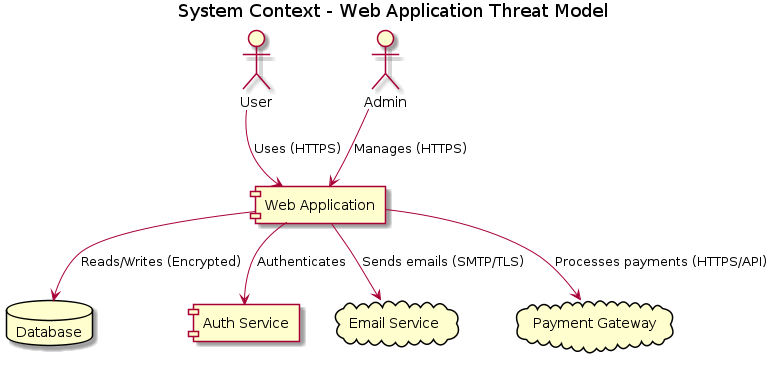
\includegraphics[width=0.8\textwidth]{images/system-context}
	\caption{PASTA Process Overview: From Business Impact to Risk Mitigation}
\end{figure}

\subsection*{Advantages and Practical Application}
\begin{itemize}
	\item Integrates business and technical perspectives for holistic risk management.
	\item Simulates attacker behavior to uncover realistic threats and attack paths.
	\item Supports risk-based decision making and prioritization of controls.\cite{uceda2015}
	\item Scalable for complex, enterprise systems and regulatory environments.
\end{itemize}

\subsection*{Implementing PASTA in the Real World}
PASTA is best suited for organizations with high-value assets, regulatory requirements, or complex threat environments. It requires cross-functional collaboration between business, security, and technical teams. Many organizations use PASTA in conjunction with automated tools for attack simulation and vulnerability scanning\cite{uceda2015,owasp}.
